\section{Constellation Orbital Parameters}
\definecolor{blue}{rgb}{0.2,0.5,0.8}

\begin{minipage}{0.5\textwidth}
\begin{tabular}{|l|c|}
	\hline
	Number of satellites & 189 \\ \hline
	Number of Planes & 9 \\ \hline
	Num. Satellites/Plane & 21 \\ \hline
	Height of the orbits (km) & 542 \\ \hline
	Constellation Type & Walker-Delta \\ \hline
	Planes Inclination & 72 \\ \hline
	Orbital Periods (min) & 95.48 \\ \hline
	Minimum Elevation (deg) & 20 \\ \hline
	Mean Pass time (min) & 4.28 \\ \hline
\end{tabular}
\end{minipage} \hfill
\begin{minipage}{0.45\textwidth}
\begin{figure}[H]
	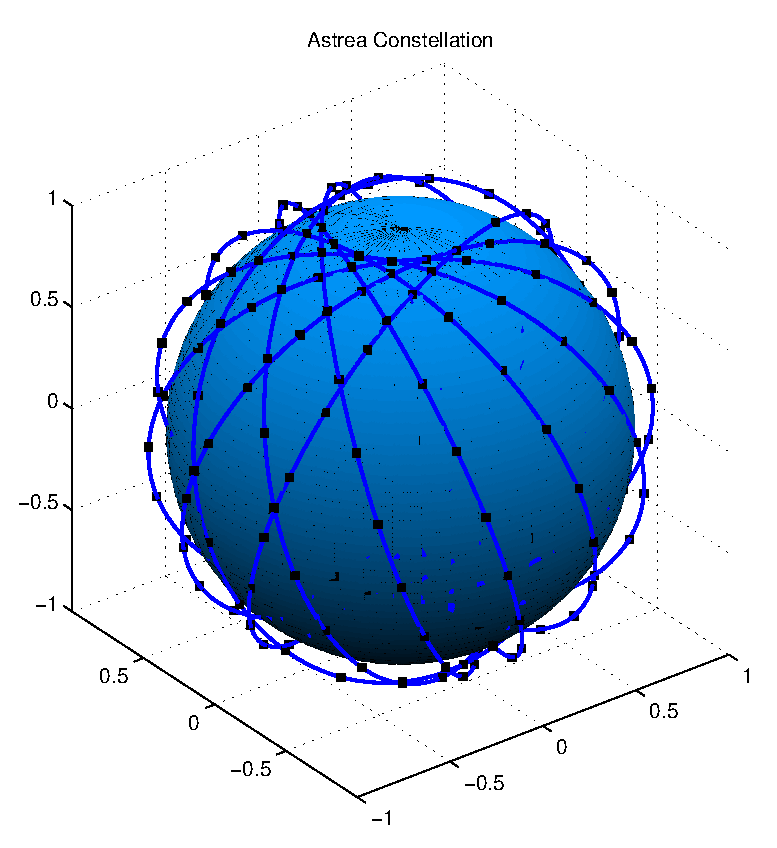
\includegraphics[scale=0.6]{ConstellationSphere}
	\caption{Spherical Distribution of the Constellation}	
\end{figure}
\end{minipage}

\begin{figure}[h]
	\centering  
	\includegraphics[scale=0.6]{ConstellationPlain}
	\caption{Ground Track Example}	
\end{figure}